\subsection{Strømforstærker}
\label{effekt_stroemforstaerker}
Strømforstærkeren opbygges som vist på figur \ref{fig:blokdiagram-stroem}. Dog vil konstantstrømsgeneratoren blive bygget i diskret elektronik. Der er valgt at der benyttes en BDX33B og en BDX34B \cite{bdx33-34-datablad} som udgangstransistorer. Dette er darlingtontransistorer, som er valgt da de har en $h_{\mathrm{FE}}$ på minimum 750 og kan klare en $I_C$ på op til 10 A. Desuden er de let tilgængelige til projektet.

\begin{figure}[h]
\centering
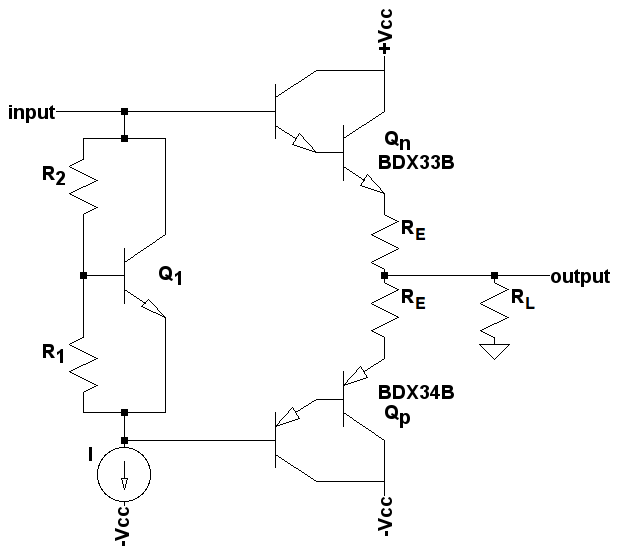
\includegraphics[scale=0.4]{teknisk/effektforstaerker/blokdiagram-stroemforstaerker.png}
\caption{Diagram over strømforstærkeren}
\label{fig:blokdiagram-stroem}
\end{figure}

Som vist, i afsnit \ref{valg_kortslutningssikring}, skal der igennem $R_{\mathrm{load}}$ løbe en $I_{\mathrm{peak}}$ på 2,24 A for at opnå en udgangseffekt på 20 W. Dette betyder desuden, som vist i udregningen i formel \ref{equ:vpeak}, at der skal være en $V_{\mathrm{peak}}$ på 17,9 V over belastningen for at afsætte 20 W. 

\begin{equation}
\label{equ:vpeak}
V_{\mathrm{peak}} = I_{\mathrm{peak}} \cdot R_{\mathrm{load}} = \mathrm{2,24~A \cdot 8~\ohm = 17,9~V}
\end{equation}

Ideelt vil en spændingsforsyning på 18 V altså være tilstrækkelig, dog er der rent praktisk behov for en større. Da de valgte darlingtontransistorer har en $V_{\mathrm{BE}}$ på op til 2,5 V, vælges forsyningsspændingen til $\pm$23 V, hvormed der også er plads til et spændingsfald over $R_E$ og en transistor i konstantstrømsgeneratoren.

\subsubsection*{Termiske forhold}
Størrelsen af $R_E$ bestemmes med udgangspunkt i at den skal skabe termisk stabilitet og til bestemmelsen af denne startes der derfor med at kigge på et termisk ækvivalentdiagram for de valgte darlingtontransistorer og de tilgængelige køleplader \cite{koeleplade-datablad}. 

\begin{figure}[h]
\centering
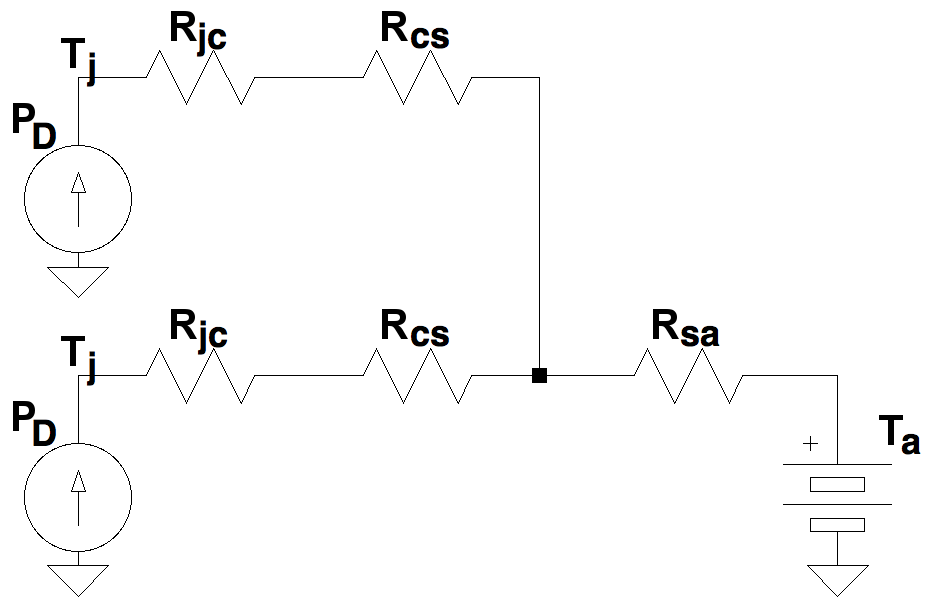
\includegraphics[scale=0.2]{teknisk/effektforstaerker/termisk_ekvivalentdiagram.png}
\caption{Termisk ækvivalentdiagram for udgangstransistorerne}
\label{fig:term-dia}
\end{figure}

På figur \ref{fig:term-dia} ses ækvivalentdiagrammet, hvor; temperatur er spænding, effekt er strøm og termisk modstand er modstand. Flere af komponenterne har samme benævnelser, da de også antager samme værdier og da der under udregningerne dermed ikke vil blive set på dem enkeltvis.\\
Størrelsen af $P_D$ er effekten afsat i en enkelt udgangstransistor og er givet ved udregningen i formel (\ref{equ:pd}) \cite{ael-mm19}. Denne formel er ganske vist givet for et klasse B udgangstrin, men den er også gældende for et klasse AB udgangstrin, da hvilestrømmem i et klasse AB udgangstrin kun er betydeligt forskellig fra nul i perioden, hvor der er et skifte i hvilken transistor, som er aktiv \cite{klasse-ab}.

\begin{equation}
\label{equ:pd}
P_D = \frac{1}{\pi^2} \cdot \frac{(V_{CC})^2}{R_{\mathrm{load}}} = \frac{1}{\pi^2} \cdot \frac{(23~\mathrm{V})^2}{8~\ohm} = 6,7~\mathrm{W}
\end{equation}

Fra darlingtontransistorernes datablad haves $R_{\mathrm{jc}} = 1,78~\tfrac{\celsius}{\mathrm{W}}$ og $T_{\mathrm{j,max}} = 150~\celsius$. Databladet for kølepladen giver $R_{\mathrm{cs}} = 1,4~\tfrac{\celsius}{\mathrm{W}}$ når der anvendes kølepasta. Fra DIN45500 \cite{DIN45500} fåes at HiFi-forstærkeren skal kunne holde til en omgivelsestemperatur på 35~\celsius, hvilket er $T_a$ i ækvivalentet. Udfra dette opstilles, ved simpel kredsløbsteori på ækvivalentkredsløbet på figur \ref{fig:term-dia}, formel (\ref{equ:tjmax}) til beregning af $R_{\mathrm{sa}}$ ved $T_j$  på sin maksimale værdi. 

\begin{equation}
\label{equ:tjmax}
T_j = T_a + P_D \cdot (R_{\mathrm{jc}} + R_{\mathrm{cs}} + 2 \cdot R_{\mathrm{sa}})
\end{equation}

Desuden opstilles udfra sikkerhedshensyn et krav om at kølepladen maksimalt må blive 40~\celsius, hvorved bestemmelse af $R_{\mathrm{sa}}$ også kan foregå ved brug af formel (\ref{equ:smax}). 

\begin{equation}
\label{equ:smax}
40~\celsius = 2 \cdot P_D \cdot R_{\mathrm{sa}}
\end{equation}

Det ses at formel (\ref{equ:smax}) bliver den afgørende betingelse og at $R_{\mathrm{sa}}$ maksimalt må være $2,99~\tfrac{\celsius}{\mathrm{W}}$. I databladet for kølepladen ses at en $R_{\mathrm{sa}}$ på $2,9~\tfrac{\celsius}{\mathrm{W}}$ kan opnåes ved en køleplade på 110 mm, hvilket derfor vælges. Størrelsen af $R_E$ kan nu bestemmes ved formel (\ref{equ:rebestem}) \cite{ael-mm19-ole-mod}% \fixme{kilde: Jan Mikkelsen, mm19, modificeret af Ole Kiel Jensen}
, hvor $K = - 2~\tfrac{\mathrm{mV}}{\celsius}$, $V_{CC} = 23$ V, $V_T = 26$ mV og $I_C = 2,24$ A.

\begin{equation}
\label{equ:rebestem}
R_E = - 2 \cdot K \cdot V_{CC} \cdot (R_{\mathrm{jc}} + R_{\mathrm{cs}} + R_{\mathrm{sa}}) - \frac{2 \cdot V_T}{I_C} = 536~\mathrm{m}\ohm
\end{equation}

\subsubsection*{Simulering af termiske forhold}

På figur \ref{fig:term-runaway} er vist en graf over effekten som bliver afsat i en af udgangstransistorerne, når der på dennes emitter sidder den beregnede $R_E$. Den lige turkis linie viser hvilken effekt den samlede køling er i stand til at lede væk, når systemet står et sted hvor omgivelsestemperaturen er 35~\celsius. Den lige grønne linie viser hvilken effekt den samlede køling er i stand til at lede væk, når systemet står et sted hvor omgivelsestemperaturen er 25~\celsius. Systemet vil, når der ikke er noget signal på indgangen, opnå en hviletemperatur svarende til skæringen mellem effektkurven for darlingtontransistoren og $"$kølingslinien$"$, altså lige over 75~\celsius~ved en omgivelsestemperatur på 35~\celsius. Havde systemet ikke indeholdt en $R_E$, eller havde denne været mindre, ville effektkurven for darlingtontransistoren ligge højere, hvormed systemet ville opnå en højere hviletemperatur. 

\begin{figure}[h]
\centering
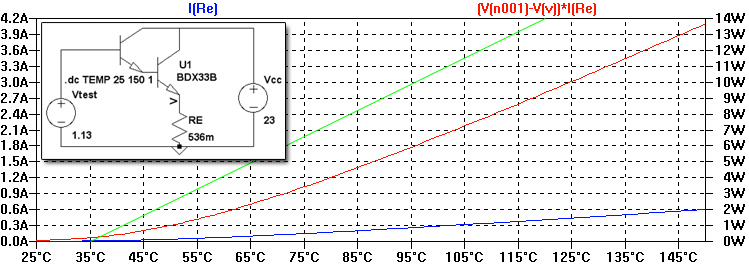
\includegraphics[width=\textwidth]{teknisk/effektforstaerker/term-runaway.png}
\caption{Graf over termiske forhold med $R_E$ og 110 mm køleplade}
\label{fig:term-runaway}
\end{figure}

Som et forsøg på at forbedre situationen beskrevet på figur \ref{fig:term-runaway}, er der på figur \ref{fig:term-runaway1} vist samme kurver, men med en køleplade på 150 mm monteret i stedet. 

\begin{figure}[h]
\centering
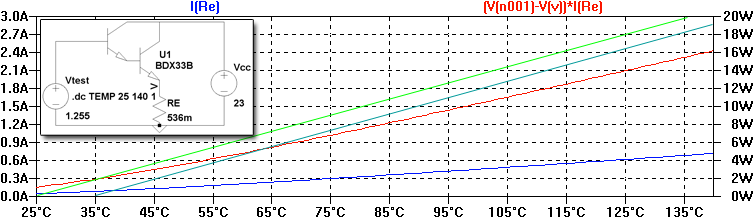
\includegraphics[width=\textwidth]{teknisk/effektforstaerker/term-runaway1.png}
\caption{Graf over termiske forhold med $R_E$ og 150 mm køleplade}
\label{fig:term-runaway1}
\end{figure}

Ved en omgivelsestemperatur på 35~\celsius~ betyder denne ændring, at darlingtontransistoren vil opnå en hviletemperatur som er over 10~\celsius~ lavere, hvilket derfor er at foretrække. Til at lave opstillingerne på figur \ref{fig:term-runaway} og \ref{fig:term-runaway1} er der antaget en hvilestrøm gennem transistoren på 45 mA. Hvilestrømmens størrelse er antaget ud fra 2 \% af peakstrømmen på udgangen, som i eksempel 13.5 i Sedra-Smith\fixme{sedra smith}.


\subsubsection*{$V_\mathrm{BE}$-multiplier}

\begin{figure}[h]
\centering
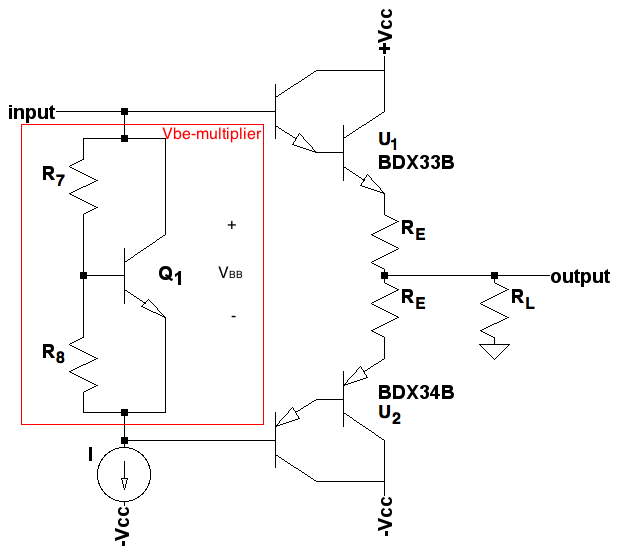
\includegraphics[scale=.4]{teknisk/effektforstaerker/vbemultiplieropbygning.png}
\caption{Strømforstærkertrinnet med markering af $V_\mathrm{be}$-multiplieren}
\label{fig:vbemulti}
\end{figure}


For at opnå en klasse AB forstærkers karakteristika skal potentialet på basis af darlingtontransistorerne hæves således det ikke er audiosignalet der skal generere den nødvendige basis-emitter-spænding for at darlingtontransistorerne åbner. Hvis ikke potentialet hæves nok vil audiosignalet blive udsat for crossoverforvrængning idet en del af signalets spændning omkring 0 V ikke vil blive overført til højtaleren. Det korrekte potentiale på basis af U1 og U2 opnås ved hjælp af en $V_\mathrm{BE}$-multiplier, hvis funktion er at opretholde et spændingsfald, $V_{BB}$, over Q1, vist på figur \ref{fig:vbemulti}. Ideelt set skal collector-emitter-spændingsfaldet over Q1 være præcis to darlington basis-emitter-spændinger, således at U1 og U2 vil åbne så snart spændingen på basis ændredes. Det anses dog ikke for at være muligt at designe kredsløbet så præcist, blandt andet på grund af tolerancerne i darlington transistorerne, som er relativt store. Derfor designes $V_\mathrm{be}$-multiplieren således at spændingsfaldet over Q1 gør at transistorerne U1 og U2 trækker en relativt lille hvilestrøm når audioinputtet er 0 V. Dermed er der sikret at U1 og U2 er åbne og at audiosignalet ikke bliver udsat for crossoverforvrængning. 


Hvilestrømmen er antaget til 45 mA i afsnittet om termiske forhold. Til Q1 benyttes en BC547B transistor, grundet at det er hvad der er til rådighed. Da der ikke er opgivet en basis-emitterspænding for darlingtontransistorerne ved en collectorstrøm på 45 mA i databladet \cite{bdx33-34-datablad} er den fundet ved hjælp af LTspice og transistorernes spicemodel. Basis-emitterspændingen blev simuleret til 1,25 V. I ligning (\ref{eq:vbbberegning}) bestemmes $V_{BB}$, som er spændingen over $V_\mathrm{BE}$-multiplieren.

\begin{equation}
V_{BB} =2 \cdot 1,25~\mathrm{V} = 2,5~\mathrm{V}
\label{eq:vbbberegning}
\end{equation}

For at opnå et spændingsfald over $V_\mathrm{BE}$-multiplieren skal der løbe en strøm. For at have kontrol over hvilken strøm der løber gennem $V_\mathrm{BE}$-multiplieren leveres denne strøm,  $I_\mathrm{bias}$, af en konstantstrømsgenerator. Generatoren er koblet på $V_\mathrm{BE}$-multiplieren som vist på figur \ref{fig:vbemulti}. Biasstrømmen skal både generere et spændingsfald over $V_\mathrm{BE}$-multiplieren og levere tilstrækkeligt basisstrøm til darlington transistorerne, således at de, ved maksimal spændingssving, ikke begrænses af $I_\mathrm{bias}$. Da der ikke vil være maksimalt signalsving på begge transistorer simultant vil der dermed kun være behov for at levere maksimal basisstrøm til én transistor af gangen. Da collectorstrømmen, $I_C$, i darlingtontransistorerne ved maksimalt signaludsving vides at være 2,24 A kan den maksimale basistrøm, $I_b$, beregnes, da der gælder at $I_b = \frac{I_C}{h_\mathrm{fe}}$. Den maksimale basisstrøm beregnes for en minimumtransistor til at være 3 mA. For at være sikker på at levere tilstrækkeligt strøm vælges $I_\mathrm{bias}$ til at være 6 mA, hvilket giver en minimumstrøm i $V_\mathrm{BE}$-multiplieren på 3 mA. Strømmen i modstandene, $R_7$ og $R_8$, ønskes at være mindre end strømmen Q1,  $I_\mathrm{c,Q1}$. Derfor vælges det at strømmen i modstandene,  $I_R$, skal være 10 gange mindre end $I_\mathrm{C,Q1}$. Dermed bliver $I_R = 0,5$ mA og $I_\mathrm{C,Q1} = 5,5$ mA.

Spændingsfaldet over $R_8$ skal være lig basis-emitterspænding for Q1 ved en collectorstrøm på 5,5 mA. Da der i databladet for en BC547B er angivet en maksimal værdi for basis-emitterspændingen på 0,7 V ved en collectorstrøm på 2 mA og 0,72 V ved en collectorstrøm på 10 mA vælges basis-emitterspændingen til at være 0,7 V. I ligning (\ref{eq:r8beregning}) beregnes $R_8$.

\begin{equation}
R_8 = \frac{V_\mathrm{BE,Q1}}{I_R} = 1,28~\mathrm{k}\ohm
\label{eq:r8beregning}
\end{equation}

Da der skal være et spændingsfald over $V_\mathrm{BE}$-multiplieren, og dermed de to modstande, på 2,5 V kan den samlede modstand $R_7$ og $R_8$ skal repræsentere beregnes hvorefter værdien af $R_7$ kan bestemmes som værende den resterende modstand når $R_8$ er trukket fra.

\begin{equation}
R_7 = \frac{V_{BB}}{I_R} - R_8 = 3,3~\mathrm{k}\ohm
\label{eq:r7beregning}
\end{equation}

En DC-analyse-simulering i LTspice viser at hvilestrømmen i strømforstærkeren bliver 55 mA. Dette passer ikke overens med beregningerne. Dog vil $V_\mathrm{BE}$-multiplieren ikke være korrekt dimensioneret hvis strømforstærkeren forsøges bygget med diskrete komponenter da tolerancerne for darlingtontransistorerne er relativt store. Derfor vil der blive indsat et potentiometer på 5 k\ohm~i stedet for $R_8$ hvorved spændingen over $V_\mathrm{BE}$-multiplieren kan gå ned til 1,16 V da sammenhængen mellem Q1's basis-emitterspænding, $R_7$ og $R_8$ er giver ved ligning (\ref{eq:vbemultipliersammenhaeng}).

\begin{equation}
V_{BB}=V_\mathrm{BE,Q1} \cdot \left( \frac{R_7}{R_8} \right)
\label{eq:vbemultipliersammenhaeng}
\end{equation}

Med potentiometeret er det dermed muligt at justere $V_{BB}$ og dermed også hvilestrømmen der løber i darlingtontransistorerne. Under implementeringen justeres potentiometeret således at hvilestrømmen stemmer overens med den beregnede.

\subsubsection*{Konstantstrømsgenerator}
Konstantstrømsgeneratorens opgave er at levere en konstant strøm. Denne strøm bruges til $V_\mathrm{BE}$-multiplieren og til spændingsforstærkeren. Som beregnet ved beregning af $V_{\mathrm{BE}}$-multiplieren skal konstantstrømsgeneratoren levere 6 mA. Opbygningen der er valgt til konstansstrømsgereratoren er afbildet på figur \ref{konstantstroemsgenerator_model}.

\begin{figure}[h]
\centering
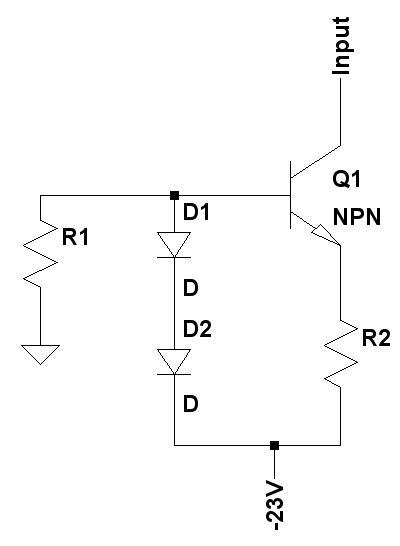
\includegraphics[scale=0.35]{teknisk/effektforstaerker/stoemgenerator.png}
\caption{Diagram der viser opbygningen af konstantstrømsgeneratoren.}
\label{konstantstroemsgenerator_model}
\end{figure}

Til konstantstrømsgeneratoren er der valgt at anvende en BC547B som transistor og en 1N4148 som diode. BC547B har en $V_\mathrm{BE}$ spænding på maksimum 720 mV \cite{bc547b-datablad}. Deraf designes det således at der er et spændingsfald på 720 mV over $D_1$, $D_2$, $R_{\mathrm{11}}$ og $Q_{9_\mathrm{BE}}$. I databladet for 1N4148 \cite{1n4148-datablad} fremgår det at den  ved en $I_F$ strøm på 8 mA har en $V_D$ spændingen på 720 mV. Strømmen igennem dioderne er givet ved hvor stor en strøm der løber igennem modstanden $R_{\mathrm{10}}$, ved den antagelse at der ses bort fra strømmen der løber ind i basen på $Q_9$. $R_{\mathrm{10}}$ er således givet ved ligning (\ref{equ:stroemgenerator_effektforstaerker1}).

\begin{equation}
\label{equ:stroemgenerator_effektforstaerker1}
R_{\mathrm{10}} = \frac{V_{CC} - 2 \cdot V_D}{I_F} = \mathrm{\frac{23~\mathrm{V} - 2 \cdot 0,72~\mathrm{V}}{8~\mathrm{mA}} = 2,7~\mathrm{k}\ohm}
\end{equation}

Da der nu ligger en konstant spænding over alle dioderne, kan man se dioden i transistoren som siddende parallelt, med det samme spændingsfald som $D_1$. Dette giver at der findes det samme, konstante, spændingsfald over $D_2$ og $R_{\mathrm{10}}$, hvilket giver en konstant strøm gennem $R_{\mathrm{11}}$. Derudfra kan $R_{\mathrm{11}}$ bestemmes når der skal løbe 6 mA i den, ved ligning (\ref{equ:stroemgenerator_effektforstaerker2}).

\begin{equation}
\label{equ:stroemgenerator_effektforstaerker2}
R_{\mathrm{11}} = \frac{V_{D}}{I_{\mathrm{const}}} = \mathrm{\frac{720~\mathrm{mV}}{6~\mathrm{mA}} = 120~\ohm}
\end{equation}

Hermed er konstantstrømsgeneratoren designet til at levere 6 mA.
